\section{C\'odigo}

\par En \textbf{main.py} usando \textit{ply} tenemos definidos el \textit{lexer} y el \textit{parser}, una funcion encargada de los tests y el programa propiamente dicho. El Lexer no merece mucha atenci\'on, as\'i que pasaremos directamente al parser:
\par Como ply utiliza LALR y \'este s\'olo permite atributos sintetizados, decidimos tener un \'unico atributo que va formando un \'arbol a medida que se hacen las reducciones. Dicho \'arbol no refleja la sintaxis, sino que es m\'as bien una representaci\'on de las posiciones y tama\~nos de los caracteres de la f\'ormula, junto con su dependencia.
\par En \textbf{Node.py} est\'a el c\'odigo de los Nodos de este \'arbol.
\par Tomando como ejemplo la producci\'on $CONCAT_1 \rightarrow CONCAT_2$ $ELEMENTS$, donde en ply se separan los terminales y no-terminales como $p[0]$ $(CONCAT_1)$, $p[1]$ $(CONCAT_2)$ y $p[2]$ $(ELEMENTS)$, lo que hacemos es $p[0] = ConcatNode(p[1], p[2])$. Es decir, representamos la concatenaci\'on de los dos no-terminales ya procesados como \'arboles en $p[1]$ y $p[2]$.
\par Por otro lado, en $GROUP \rightarrow \{ E \}$, tenemos $p[0]$ $(GROUP)$, $p[1]$ $(\{)$, $p[2]$ $(E)$ y $p[3]$ $(\})$, y en este caso pasamos directamente el \'arbol procesado en $p[2]$. Es decir, $p[0] = p[2]$, ya que no hay ning\'un cambio respecto a la posicion o tama\~no.
\par Estos dos ejemplos muestran que el \'arbol que generamos tiende a ser sint\'actico pero no lo es necesariamente. De hecho, definimos un \texttt{LineNode} que representa la l\'inea de divisi\'on, y que se instancia en la implementaci\'on de \texttt{DivideNode}.
\par Finalmente, en la producci\'on $S \rightarrow E$ simplemente completamos el \'arbol con la ra\'iz y llamamos al m\'etodo $toSvg()$ de \'esta. $p[0] = MainNode(p[1]).toSvg()$, donde $MainNode$ representa la ra\'iz del \'arbol y $toSvg()$ va generando y concatenando los $toSvg$ de los subnodos para obtener el svg final de la f\'ormula.

\par \phantom{a}
\par A continuaci\'on inclu\'imos unos ejemplos de resultados obtenidos y luego presentamos el c\'odigo de \textbf{main.py} y \textbf{Node.py}:

\newpage
\subsection{Ejemplos}
\begin{figure}[htbp]
	\centering
	\begin{subfigure}[b]{0.3\textwidth}
	  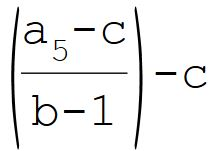
\includegraphics[width=\textwidth]{imgs/test1}
	  \caption{$(a \_ 5-c/b-1)-c$}
	\end{subfigure}
	\quad
	\begin{subfigure}[b]{0.3\textwidth}
	  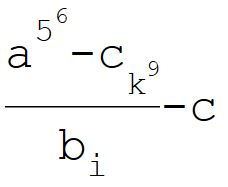
\includegraphics[width=\textwidth]{imgs/test2}
	  \caption{$\{a \wedge \{5 \wedge 6\}-c \_ \{k \wedge 9\}/b \_ i\}-c$}
	\end{subfigure}
	\quad
	\begin{subfigure}[b]{0.3\textwidth}
	  \includegraphics[width=\textwidth]{imgs/test3}
	  \caption{$(A \wedge BC \wedge D/E \wedge F \_ G+H)-I$}
	\end{subfigure}
	
	\hfill
	
	\hfill
	
	\hfill
	
	\begin{subfigure}[b]{\textwidth}
	  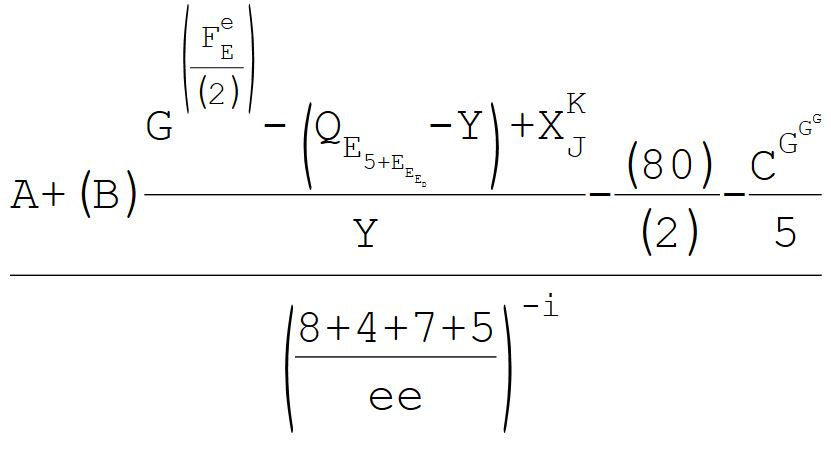
\includegraphics[width=\textwidth]{imgs/test4}
	  \caption{$A+(B)\{G \wedge \{(F \wedge e \_ E/(2))\}-(Q \_ \{E \_ \{\{5\}+E \_ \{E \_ \{E \_ D\}\}\}\}-Y)+X \wedge K \_ J/Y\}-\{(80)/(2)\}-\{C \wedge \{G \wedge \{G \wedge \{G\}\}\}/5\}/(\{8+4+7\}+5/ee) \wedge \{-i\}$}
	\end{subfigure}
\end{figure}

\newpage
\subsection{main.py}
\lstinputlisting{../src/main.py}

\newpage
\subsection{Node.py}
\lstinputlisting{../src/Node.py}